\documentclass[tikz,margin=2mm]{standalone}
\pagestyle{empty}

%\usepackage{aistats2020}
\usepackage{amsmath}
\usepackage{bm}
\usetikzlibrary{positioning,calc, arrows}

% variable styles
\tikzstyle{error} = [ draw=black,fill=gray!50!white,circle, inner sep = 1pt, minimum size = 0.35cm ]
\tikzstyle{latent} = [ draw, circle, inner sep = 2pt, minimum size = 0.65cm ]
\tikzstyle{observed} = [ draw, rectangle, inner sep = 2pt, minimum size = 0.65cm ]
\tikzstyle{measure} = [ draw, rectangle, inner sep = 0pt, minimum size = 0.45cm, outer sep = 0.5pt]
\tikzstyle{refpoint} = [inner sep = 0pt, outer sep = 0pt]


\tikzstyle{edge} = [->]
\tikzstyle{highlightEdge} = [->, very thick]
\tikzstyle{highlightEdge2} = [->, dashed]
\tikzstyle{transform} = [->, very thick, >=triangle 45]

\begin{document}

% Page 1: Democracy example from Bollen 1996
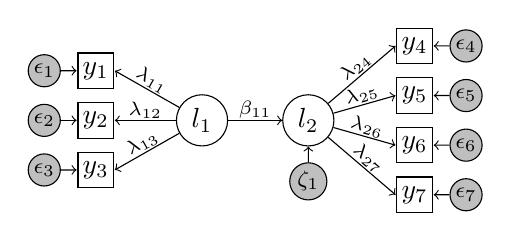
\begin{tikzpicture}[scale=0.9]
	\node[latent] (xi1) at (1.5, 0) {$ \l_1 $};
	\node[latent] (eta1) at (3, 0) {$ \l_2 $};
	\node[measure] (x1) at ( 0, 0.7) {$ y_1 $};
	\node[measure] (x2) at ( 0, 0) {$ y_2 $};
	\node[measure] (x3) at ( 0, -0.7) {$ y_3 $};
	\node[measure] (y1) at ( 4.5, 1.05) {$ y_4 $};
	\node[measure] (y2) at ( 4.5, 0.35) {$ y_5 $};
	\node[measure] (y3) at ( 4.5, -0.35) {$ y_6 $};
	\node[measure] (y4) at ( 4.5, -1.05) {$ y_7 $};

	\node[error] (zeta1) [below=.2cm of eta1] {\footnotesize $ \zeta_1 $};
	\node[error] (e1) [right=.2cm of y1] {\footnotesize $ \epsilon_4 $};
	\node[error] (e2) [right=.2cm of y2] {\footnotesize $ \epsilon_5 $};
	\node[error] (e3) [right=.2cm of y3] {\footnotesize $ \epsilon_6 $};
	\node[error] (e4) [right=.2cm of y4] {\footnotesize $ \epsilon_7 $};
	\node[error] (d1) [left=.2cm of x1] {\footnotesize $ \epsilon_1 $};
	\node[error] (d2) [left=.2cm of x2] {\footnotesize $ \epsilon_2 $};
	\node[error] (d3) [left=.2cm of x3] {\footnotesize $ \epsilon_3 $};

	\draw[edge](xi1) -- (eta1) node[midway, above, sloped, yshift=-0.1cm]{\scriptsize $ \beta_{11} $};
	\draw[edge](xi1) -- (x1.east) node[midway, above, sloped, yshift=-0.1cm]{\scriptsize $ \lambda_{11} $};
	\draw[edge](xi1) -- (x2.east) node[midway, above, sloped, yshift=-0.1cm]{\scriptsize $ \lambda_{12} $};
	\draw[edge](xi1) -- (x3.east) node[midway, above, sloped, yshift=-0.1cm]{\scriptsize $ \lambda_{13} $};
	\draw[edge](eta1) -- (y1.west) node[midway, above, sloped, yshift=-0.1cm]{\scriptsize $ \lambda_{24} $};
	\draw[edge](eta1) -- (y2.west) node[midway, above, sloped, yshift=-0.1cm]{\scriptsize $ \lambda_{25} $};
	\draw[edge](eta1) -- (y3.west) node[midway, above, sloped, yshift=-0.1cm]{\scriptsize $ \lambda_{26} $};
	\draw[edge](eta1) -- (y4.west) node[midway, above, sloped, yshift=-0.1cm]{\scriptsize $ \lambda_{27} $};
	\draw[edge](e1) -- (y1);
	\draw[edge](e2) -- (y2);
	\draw[edge](e3) -- (y3);
	\draw[edge](e4) -- (y4);
	\draw[edge](d1) -- (x1);
	\draw[edge](d2) -- (x2);
	\draw[edge](d3) -- (x3);
	\draw[edge](zeta1) -- (eta1);

\end{tikzpicture}


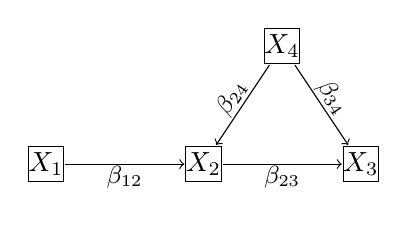
\begin{tikzpicture}[scale=1]
	\node[measure] (x1) at ( 0, 0 ) { $ X_1 $ };
	\node[measure] (x2) at ( 2, 0 ) { $ X_2 $ };
	\node[measure] (x3) at ( 4, 0 ) { $ X_3 $ };
	\node[measure] (x4) at ( 3, 1.5 ) { $ X_4 $ };

	\draw[edge](x1) -- (x2) node[midway, below, yshift=0.1cm]{\small $\beta_{12}$};
	\draw[edge](x2) -- (x3) node[midway, below, yshift=0.1cm]{\small $\beta_{23}$};
	\draw[edge](x4) -- (x2) node[midway, above, sloped, yshift=-0.1cm]{\small $\beta_{24}$};
	\draw[edge](x4) -- (x3) node[midway, above, sloped, yshift=-0.1cm]{\small $\beta_{34}$};

\end{tikzpicture}
\end{document}
